%%%%%%%%%%%%%%%%%%%%%%%%%%%%%%%%%%%%%%%%%
% Important note:
% Chapter heading images should have a 2:1 width:height ratio,
% e.g. 920px width and 460px height.
%
%%%%%%%%%%%%%%%%%%%%%%%%%%%%%%%%%%%%%%%%%


%----------------------------------------------------------------------------------------
%	PACKAGES AND OTHER DOCUMENT CONFIGURATIONS
%----------------------------------------------------------------------------------------

\documentclass[openany,11pt,fleqn]{book} % Default font size and left-justified equations

\usepackage[top=3cm,bottom=3cm,left=3.2cm,right=3.2cm,headsep=10pt,letterpaper]{geometry} % Page margins

\usepackage{xcolor} % Required for specifying colors by name
\definecolor{ocre}{RGB}{52,177,201} % Define the orange color used for highlighting throughout the book

% Font Settings
\usepackage{avant} % Use the Avantgarde font for headings
%\usepackage{times} % Use the Times font for headings
\usepackage{mathptmx} % Use the Adobe Times Roman as the default text font together with math symbols from the Sym­bol, Chancery and Com­puter Modern fonts
\usepackage{microtype} % Slightly tweak font spacing for aesthetics
\usepackage[utf8]{inputenc} % Required for including letters with accents
\usepackage[T1]{fontenc} % Use 8-bit encoding that has 256 glyphs
\usepackage{amsthm}

\usepackage{mathtools}

\usepackage{minted}

\usepackage{tikz}
\usepackage{pgfplots}
\usepgfplotslibrary{fillbetween}
\usepackage{multirow}
\usepackage{array}
\usetikzlibrary{arrows.meta, positioning, calc, trees, shapes, decorations, matrix, fit}

% Bibliography
\usepackage[style=alphabetic,sorting=nyt,sortcites=true,autopunct=true,babel=hyphen,hyperref=true,abbreviate=false,backref=true,backend=biber]{biblatex}
\addbibresource{bibliography.bib} % BibTeX bibliography file
\defbibheading{bibempty}{}
\usepackage{float}


%----------------------------------------------------------------------------------------
%	VARIOUS REQUIRED PACKAGES
%----------------------------------------------------------------------------------------

\usepackage{titlesec} % Allows customization of titles

\usepackage{graphicx} % Required for including pictures
\graphicspath{{Pictures/}} % Specifies the directory where pictures are stored
% \graphicspath{{Plots/}}
\usepackage{lipsum} % Inserts dummy text

\usepackage{tikz} % Required for drawing custom shapes

\usepackage[english]{babel} % English language/hyphenation

\usepackage{enumitem} % Customize lists
\setlist{nolistsep} % Reduce spacing between bullet points and numbered lists

\usepackage{booktabs} % Required for nicer horizontal rules in tables

\usepackage{eso-pic} % Required for specifying an image background in the title page

%----------------------------------------------------------------------------------------
%	MAIN TABLE OF CONTENTS
%----------------------------------------------------------------------------------------

\usepackage{titletoc} % Required for manipulating the table of contents

\contentsmargin{0cm} % Removes the default margin
% Chapter text styling
\titlecontents{chapter}[1.25cm] % Indentation
{\addvspace{15pt}\large\sffamily\bfseries} % Spacing and font options for chapters
{\color{ocre!60}\contentslabel[\thecontentslabel]{2cm}\color{ocre}} % Chapter number
{}  
{\color{ocre!60}\normalsize\sffamily\bfseries\;\titlerule*[.5pc]{.}\;\thecontentspage} % Page number
% Section text styling
\titlecontents{section}[1.25cm] % Indentation
{\addvspace{5pt}\sffamily\bfseries} % Spacing and font options for sections
{\contentslabel[\thecontentslabel]{1.25cm}} % Section number
{}
{\sffamily\hfill\color{black}\thecontentspage} % Page number
[]
% Subsection text styling
\titlecontents{subsection}[1.25cm] % Indentation
{\addvspace{1pt}\sffamily\small} % Spacing and font options for subsections
{\contentslabel[\thecontentslabel]{1.25cm}} % Subsection number
{}
{\sffamily\;\titlerule*[.5pc]{.}\;\thecontentspage} % Page number
[] 

%----------------------------------------------------------------------------------------
%	MINI TABLE OF CONTENTS IN CHAPTER HEADS
%----------------------------------------------------------------------------------------

% Section text styling
\titlecontents{lsection}[0em] % Indendating
{\footnotesize\sffamily} % Font settings
{}
{}
{}

% Subsection text styling
\titlecontents{lsubsection}[.5em] % Indentation
{\normalfont\footnotesize\sffamily} % Font settings
{}
{}
{}
 
%----------------------------------------------------------------------------------------
%	PAGE HEADERS
%----------------------------------------------------------------------------------------

\usepackage{fancyhdr} % Required for header and footer configuration

\pagestyle{fancy}
\renewcommand{\chaptermark}[1]{\markboth{\sffamily\normalsize\bfseries\chaptername\ \thechapter.\ #1}{}} % Chapter text font settings
\renewcommand{\sectionmark}[1]{\markright{\sffamily\normalsize\thesection\hspace{5pt}#1}{}} % Section text font settings
\fancyhf{} \fancyhead[LE,RO]{\sffamily\normalsize\thepage} % Font setting for the page number in the header
\fancyhead[LO]{\rightmark} % Print the nearest section name on the left side of odd pages
\fancyhead[RE]{\leftmark} % Print the current chapter name on the right side of even pages
\renewcommand{\headrulewidth}{0.5pt} % Width of the rule under the header
\addtolength{\headheight}{2.5pt} % Increase the spacing around the header slightly
\renewcommand{\footrulewidth}{0pt} % Removes the rule in the footer
\fancypagestyle{plain}{\fancyhead{}\renewcommand{\headrulewidth}{0pt}} % Style for when a plain pagestyle is specified

% Removes the header from odd empty pages at the end of chapters
\makeatletter
\renewcommand{\cleardoublepage}{
\clearpage\ifodd\c@page\else
\hbox{}
\vspace*{\fill}
\thispagestyle{empty}
\newpage
\fi}

%----------------------------------------------------------------------------------------
%	THEOREM STYLES
%----------------------------------------------------------------------------------------

\usepackage{amsmath,amsfonts,amssymb,amsthm} % For math equations, theorems, symbols, etc

\newcommand{\intoo}[2]{\mathopen{]}#1\,;#2\mathclose{[}}
\newcommand{\ud}{\mathop{\mathrm{{}d}}\mathopen{}}
\newcommand{\intff}[2]{\mathopen{[}#1\,;#2\mathclose{]}}
\newtheorem{notation}{Notation}[chapter]

%%%%%%%%%%%%%%%%%%%%%%%%%%%%%%%%%%%%%%%%%%%%%%%%%%%%%%%%%%%%%%%%%%%%%%%%%%%
%%%%%%%%%%%%%%%%%%%% dedicated to boxed/framed environements %%%%%%%%%%%%%%
%%%%%%%%%%%%%%%%%%%%%%%%%%%%%%%%%%%%%%%%%%%%%%%%%%%%%%%%%%%%%%%%%%%%%%%%%%%
\newtheoremstyle{ocrenumbox}% % Theorem style name
{0pt}% Space above
{0pt}% Space below
{\normalfont}% % Body font
{}% Indent amount
{\small\bf\sffamily\color{ocre}}% % Theorem head font
{\;}% Punctuation after theorem head
{0.25em}% Space after theorem head
{\small\sffamily\color{ocre}\thmname{#1}\nobreakspace\thmnumber{\@ifnotempty{#1}{}\@upn{#2}}% Theorem text (e.g. Theorem 2.1)
\thmnote{\nobreakspace\the\thm@notefont\sffamily\bfseries\color{black}---\nobreakspace#3.}} % Optional theorem note
\renewcommand{\qedsymbol}{$\blacksquare$}% Optional qed square

\newtheoremstyle{blacknumex}% Theorem style name
{5pt}% Space above
{5pt}% Space below
{\normalfont}% Body font
{} % Indent amount
{\small\bf\sffamily}% Theorem head font
{\;}% Punctuation after theorem head
{0.25em}% Space after theorem head
{\small\sffamily{\tiny\ensuremath{\blacksquare}}\nobreakspace\thmname{#1}\nobreakspace\thmnumber{\@ifnotempty{#1}{}\@upn{#2}}% Theorem text (e.g. Theorem 2.1)
\thmnote{\nobreakspace\the\thm@notefont\sffamily\bfseries---\nobreakspace#3.}}% Optional theorem note

\newtheoremstyle{blacknumbox} % Theorem style name
{0pt}% Space above
{0pt}% Space below
{\normalfont}% Body font
{}% Indent amount
{\small\bf\sffamily}% Theorem head font
{\;}% Punctuation after theorem head
{0.25em}% Space after theorem head
{\small\sffamily\thmname{#1}\nobreakspace\thmnumber{\@ifnotempty{#1}{}\@upn{#2}}% Theorem text (e.g. Theorem 2.1)
\thmnote{\nobreakspace\the\thm@notefont\sffamily\bfseries---\nobreakspace#3.}}% Optional theorem note

%%%%%%%%%%%%%%%%%%%%%%%%%%%%%%%%%%%%%%%%%%%%%%%%%%%%%%%%%%%%%%%%%%%%%%%%%%%
%%%%%%%%%%%%% dedicated to non-boxed/non-framed environements %%%%%%%%%%%%%
%%%%%%%%%%%%%%%%%%%%%%%%%%%%%%%%%%%%%%%%%%%%%%%%%%%%%%%%%%%%%%%%%%%%%%%%%%%
\newtheoremstyle{ocrenum}% % Theorem style name
{5pt}% Space above
{5pt}% Space below
{\normalfont}% % Body font
{}% Indent amount
{\small\bf\sffamily\color{ocre}}% % Theorem head font
{\;}% Punctuation after theorem head
{0.25em}% Space after theorem head
{\small\sffamily\color{ocre}\thmname{#1}\nobreakspace\thmnumber{\@ifnotempty{#1}{}\@upn{#2}}% Theorem text (e.g. Theorem 2.1)
\thmnote{\nobreakspace\the\thm@notefont\sffamily\bfseries\color{black}---\nobreakspace#3.}} % Optional theorem note
\renewcommand{\qedsymbol}{$\blacksquare$}% Optional qed square
\makeatother

% Defines the theorem text style for each type of theorem to one of the three styles above
\newcounter{dummy} 
\numberwithin{dummy}{section}
\theoremstyle{ocrenumbox}


\newtheorem{theoremeT}[dummy]{Theorem}
\newtheorem{lemma}[dummy]{Lemma}
\newtheorem{observation}[dummy]{Observation}
\newtheorem{proposition}[dummy]{Proposition}
% \newtheorem{definition}[dummy]{Definition}
\newtheorem{claim}[dummy]{Claim}
\newtheorem{fact}[dummy]{Fact}
\newtheorem{assumption}[dummy]{Assumption}

\newtheorem{problem}{Problem}[chapter]
% \newtheorem{exercise}{Exercise}[chapter]
\theoremstyle{blacknumex}
\newtheorem{exampleT}{Example}[chapter]
\theoremstyle{blacknumbox}
\newtheorem{vocabulary}{Vocabulary}[chapter]
\newtheorem{definitionT}{Definition}[section]
\newtheorem{corollaryT}[dummy]{Corollary}
\theoremstyle{ocrenum}



%----------------------------------------------------------------------------------------
%	DEFINITION OF COLORED BOXES
%----------------------------------------------------------------------------------------

\RequirePackage[framemethod=default]{mdframed} % Required for creating the theorem, definition, exercise and corollary boxes

% Theorem box
\newmdenv[skipabove=7pt,
skipbelow=7pt,
backgroundcolor=black!5,
linecolor=ocre,
innerleftmargin=5pt,
innerrightmargin=5pt,
innertopmargin=5pt,
leftmargin=0cm,
rightmargin=0cm,
innerbottommargin=5pt]{tBox}

% Exercise box	  
\newmdenv[skipabove=7pt,
skipbelow=7pt,
rightline=false,
leftline=true,
topline=false,
bottomline=false,
backgroundcolor=ocre!10,
linecolor=ocre,
innerleftmargin=5pt,
innerrightmargin=5pt,
innertopmargin=5pt,
innerbottommargin=5pt,
leftmargin=0cm,
rightmargin=0cm,
linewidth=4pt]{eBox}	

% Definition box
\newmdenv[skipabove=7pt,
skipbelow=7pt,
rightline=false,
leftline=true,
topline=false,
bottomline=false,
linecolor=ocre,
innerleftmargin=5pt,
innerrightmargin=5pt,
innertopmargin=0pt,
leftmargin=0cm,
rightmargin=0cm,
linewidth=4pt,
innerbottommargin=0pt]{dBox}	

% Corollary box
\newmdenv[skipabove=7pt,
skipbelow=7pt,
rightline=false,
leftline=true,
topline=false,
bottomline=false,
linecolor=gray,
backgroundcolor=black!5,
innerleftmargin=5pt,
innerrightmargin=5pt,
innertopmargin=5pt,
leftmargin=0cm,
rightmargin=0cm,
linewidth=4pt,
innerbottommargin=5pt]{cBox}

% Creates an environment for each type of theorem and assigns it a theorem text style from the "Theorem Styles" section above and a colored box from above
\newenvironment{theorem}{\begin{tBox}\begin{theoremeT}}{\end{theoremeT}\end{tBox}}
\newenvironment{exercise}{\begin{eBox}\begin{exerciseT}}{\hfill{\color{ocre}\tiny\ensuremath{\blacksquare}}\end{exerciseT}\end{eBox}}				  
\newenvironment{definition}{\begin{dBox}\begin{definitionT}}{\end{definitionT}\end{dBox}}	
\newenvironment{example}{\begin{exampleT}}{\hfill{\tiny\ensuremath{\blacksquare}}\end{exampleT}}		
\newenvironment{corollary}{\begin{cBox}\begin{corollaryT}}{\end{corollaryT}\end{cBox}}	

%----------------------------------------------------------------------------------------
%	REMARK ENVIRONMENT
%----------------------------------------------------------------------------------------

\newenvironment{remark}{\par\vspace{10pt}\small % Vertical white space above the remark and smaller font size
\begin{list}{}{
\leftmargin=35pt % Indentation on the left
\rightmargin=25pt}\item\ignorespaces % Indentation on the right
\makebox[-2.5pt]{\begin{tikzpicture}[overlay]
\node[draw=ocre!60,line width=1pt,circle,fill=ocre!25,font=\sffamily\bfseries,inner sep=2pt,outer sep=0pt] at (-15pt,0pt){\textcolor{ocre}{R}};\end{tikzpicture}} % Orange R in a circle
\advance\baselineskip -1pt}{\end{list}\vskip5pt} % Tighter line spacing and white space after remark

%----------------------------------------------------------------------------------------
%	SECTION NUMBERING IN THE MARGIN
%----------------------------------------------------------------------------------------

\makeatletter
\renewcommand{\@seccntformat}[1]{\llap{\textcolor{ocre}{\csname the#1\endcsname}\hspace{1em}}}                    
\renewcommand{\section}{\@startsection{section}{1}{\z@}
{-4ex \@plus -1ex \@minus -.4ex}
{1ex \@plus.2ex }
{\normalfont\large\sffamily\bfseries}}
\renewcommand{\subsection}{\@startsection {subsection}{2}{\z@}
{-3ex \@plus -0.1ex \@minus -.4ex}
{0.5ex \@plus.2ex }
{\normalfont\sffamily\bfseries}}
\renewcommand{\subsubsection}{\@startsection {subsubsection}{3}{\z@}
{-2ex \@plus -0.1ex \@minus -.2ex}
{.2ex \@plus.2ex }
{\normalfont\small\sffamily\bfseries}}                        
\renewcommand\paragraph{\@startsection{paragraph}{4}{\z@}
{-2ex \@plus-.2ex \@minus .2ex}
{.1ex}
{\normalfont\small\sffamily\bfseries}}

%----------------------------------------------------------------------------------------
%	HYPERLINKS IN THE DOCUMENTS
%----------------------------------------------------------------------------------------

% For an unclear reason, the package should be loaded now and not later
\usepackage{hyperref}
\hypersetup{hidelinks,backref=true,pagebackref=true,hyperindex=true,colorlinks=false,breaklinks=true,urlcolor= ocre,bookmarks=true,bookmarksopen=false,pdftitle={Title},pdfauthor={Author}}

%----------------------------------------------------------------------------------------
%	CHAPTER HEADINGS
%----------------------------------------------------------------------------------------

% The set-up below should be (sadly) manually adapted to the overall margin page septup controlled by the geometry package loaded in the main.tex document. It is possible to implement below the dimensions used in the goemetry package (top,bottom,left,right)... TO BE DONE

\newcommand{\thechapterimage}{}
\newcommand{\chapterimage}[1]{\renewcommand{\thechapterimage}{#1}}

% Numbered chapters with mini tableofcontents
\def\thechapter{\arabic{chapter}}
\def\@makechapterhead#1{
\thispagestyle{empty}
{\centering \normalfont\sffamily
\ifnum \c@secnumdepth >\m@ne
\if@mainmatter
\startcontents
\begin{tikzpicture}[remember picture,overlay]
\node at (current page.north west)
{\begin{tikzpicture}[remember picture,overlay]
\node[anchor=north west,inner sep=0pt] at (0,0) {\includegraphics[width=\paperwidth]{\thechapterimage}};
%%%%%%%%%%%%%%%%%%%%%%%%%%%%%%%%%%%%%%%%%%%%%%%%%%%%%%%%%%%%%%%%%%%%%%%%%%%%%%%%%%%%%
% Commenting the 3 lines below removes the small contents box in the chapter heading
%\fill[color=ocre!10!white,opacity=.6] (1cm,0) rectangle (8cm,-7cm);
%\node[anchor=north west] at (1.1cm,.35cm) {\parbox[t][8cm][t]{6.5cm}{\huge\bfseries\flushleft \printcontents{l}{1}{\setcounter{tocdepth}{2}}}};
\draw[anchor=west] (5cm,-9cm) node [rounded corners=20pt,fill=ocre!10!white,text opacity=1,draw=ocre,draw opacity=1,line width=1.5pt,fill opacity=.6,inner sep=12pt]{\Large\sffamily\bfseries\textcolor{black}{\thechapter. #1\strut\makebox[22cm]{}}};
%%%%%%%%%%%%%%%%%%%%%%%%%%%%%%%%%%%%%%%%%%%%%%%%%%%%%%%%%%%%%%%%%%%%%%%%%%%%%%%%%%%%%
\end{tikzpicture}};
\end{tikzpicture}}
\vskip 223pt % Changed to \vskip from \par\vspace*{} bc it was skipping pages for me
\fi
\fi}

% Unnumbered chapters without mini tableofcontents (could be added though) 
\def\@makeschapterhead#1{
\thispagestyle{empty}
{\centering \normalfont\sffamily
\ifnum \c@secnumdepth >\m@ne
\if@mainmatter
\begin{tikzpicture}[remember picture,overlay]
\node at (current page.north west)
{\begin{tikzpicture}[remember picture,overlay]
\node[anchor=north west,inner sep=0pt] at (0,0) {\includegraphics[width=\paperwidth]{\thechapterimage}};
\draw[anchor=west] (5cm,-9cm) node [rounded corners=20pt,fill=ocre!10!white,fill opacity=.6,inner sep=12pt,text opacity=1,draw=ocre,draw opacity=1,line width=1.5pt]{\huge\sffamily\bfseries\textcolor{black}{#1\strut\makebox[22cm]{}}};
\end{tikzpicture}};
\end{tikzpicture}}
\vskip 223pt % Changed to \vskip from \par\vspace*{} bc it was skipping pages for me
\fi
\fi
}
\makeatother % Insert the commands.tex file which contains the majority of the structure behind the template

%----------------------------------------------------------------------------------------
%	Definitions of new commands
%----------------------------------------------------------------------------------------

\newcounter{ttl@toc@default} % Add counter definition

\newcommand{\cvx}{convex}
\thinmuskip=6mu
\medmuskip=8mu plus 4mu minus 6mu
\thickmuskip=10mu plus 10mu
\setlength{\parindent}{0pt} % Remove paragraph indentation
\setlength{\parskip}{0pt} % Remove paragraph skip
\allowdisplaybreaks

\includeonly{
    LECTURE_1/lecture_1.tex,
    % LECTURE_2/lecture_2.tex,
    % LECTURE_3/lecture_3.tex,
    % LECTURE_4/lecture_4.tex,
    % LECTURE_5/lecture_5.tex,
    % LECTURE_6/lecture_6.tex
}

\begin{document}

\renewcommand{\thedummy}{\Roman{chapter}.\Roman{section}.\Roman{dummy}}
\renewcommand{\thedefinitionT}{\Roman{chapter}.\Roman{section}.\Roman{definitionT}}
\renewcommand{\theexampleT}{\Roman{chapter}.\Roman{exampleT}}
\renewcommand{\thechapter}{Lecture \Roman{chapter}} % Chapter numbering in Roman numerals
\renewcommand{\thesection}{\Roman{chapter}.\Roman{section}} % Section numbering in Roman numerals
\renewcommand{\thesubsection}{\Roman{chapter}.\Roman{section}.\Roman{subsection}} % Subsection numbering in Roman numerals
\renewcommand{\thetable}{\Roman{chapter}.\Roman{table}}
\renewcommand{\theequation}{\Roman{chapter}.\Roman{equation}}
\renewcommand{\theproblem}{\Roman{problem}}


%----------------------------------------------------------------------------------------
%	TITLE PAGE
%----------------------------------------------------------------------------------------

\begingroup
\thispagestyle{empty}
\AddToShipoutPicture*{\put(0,0){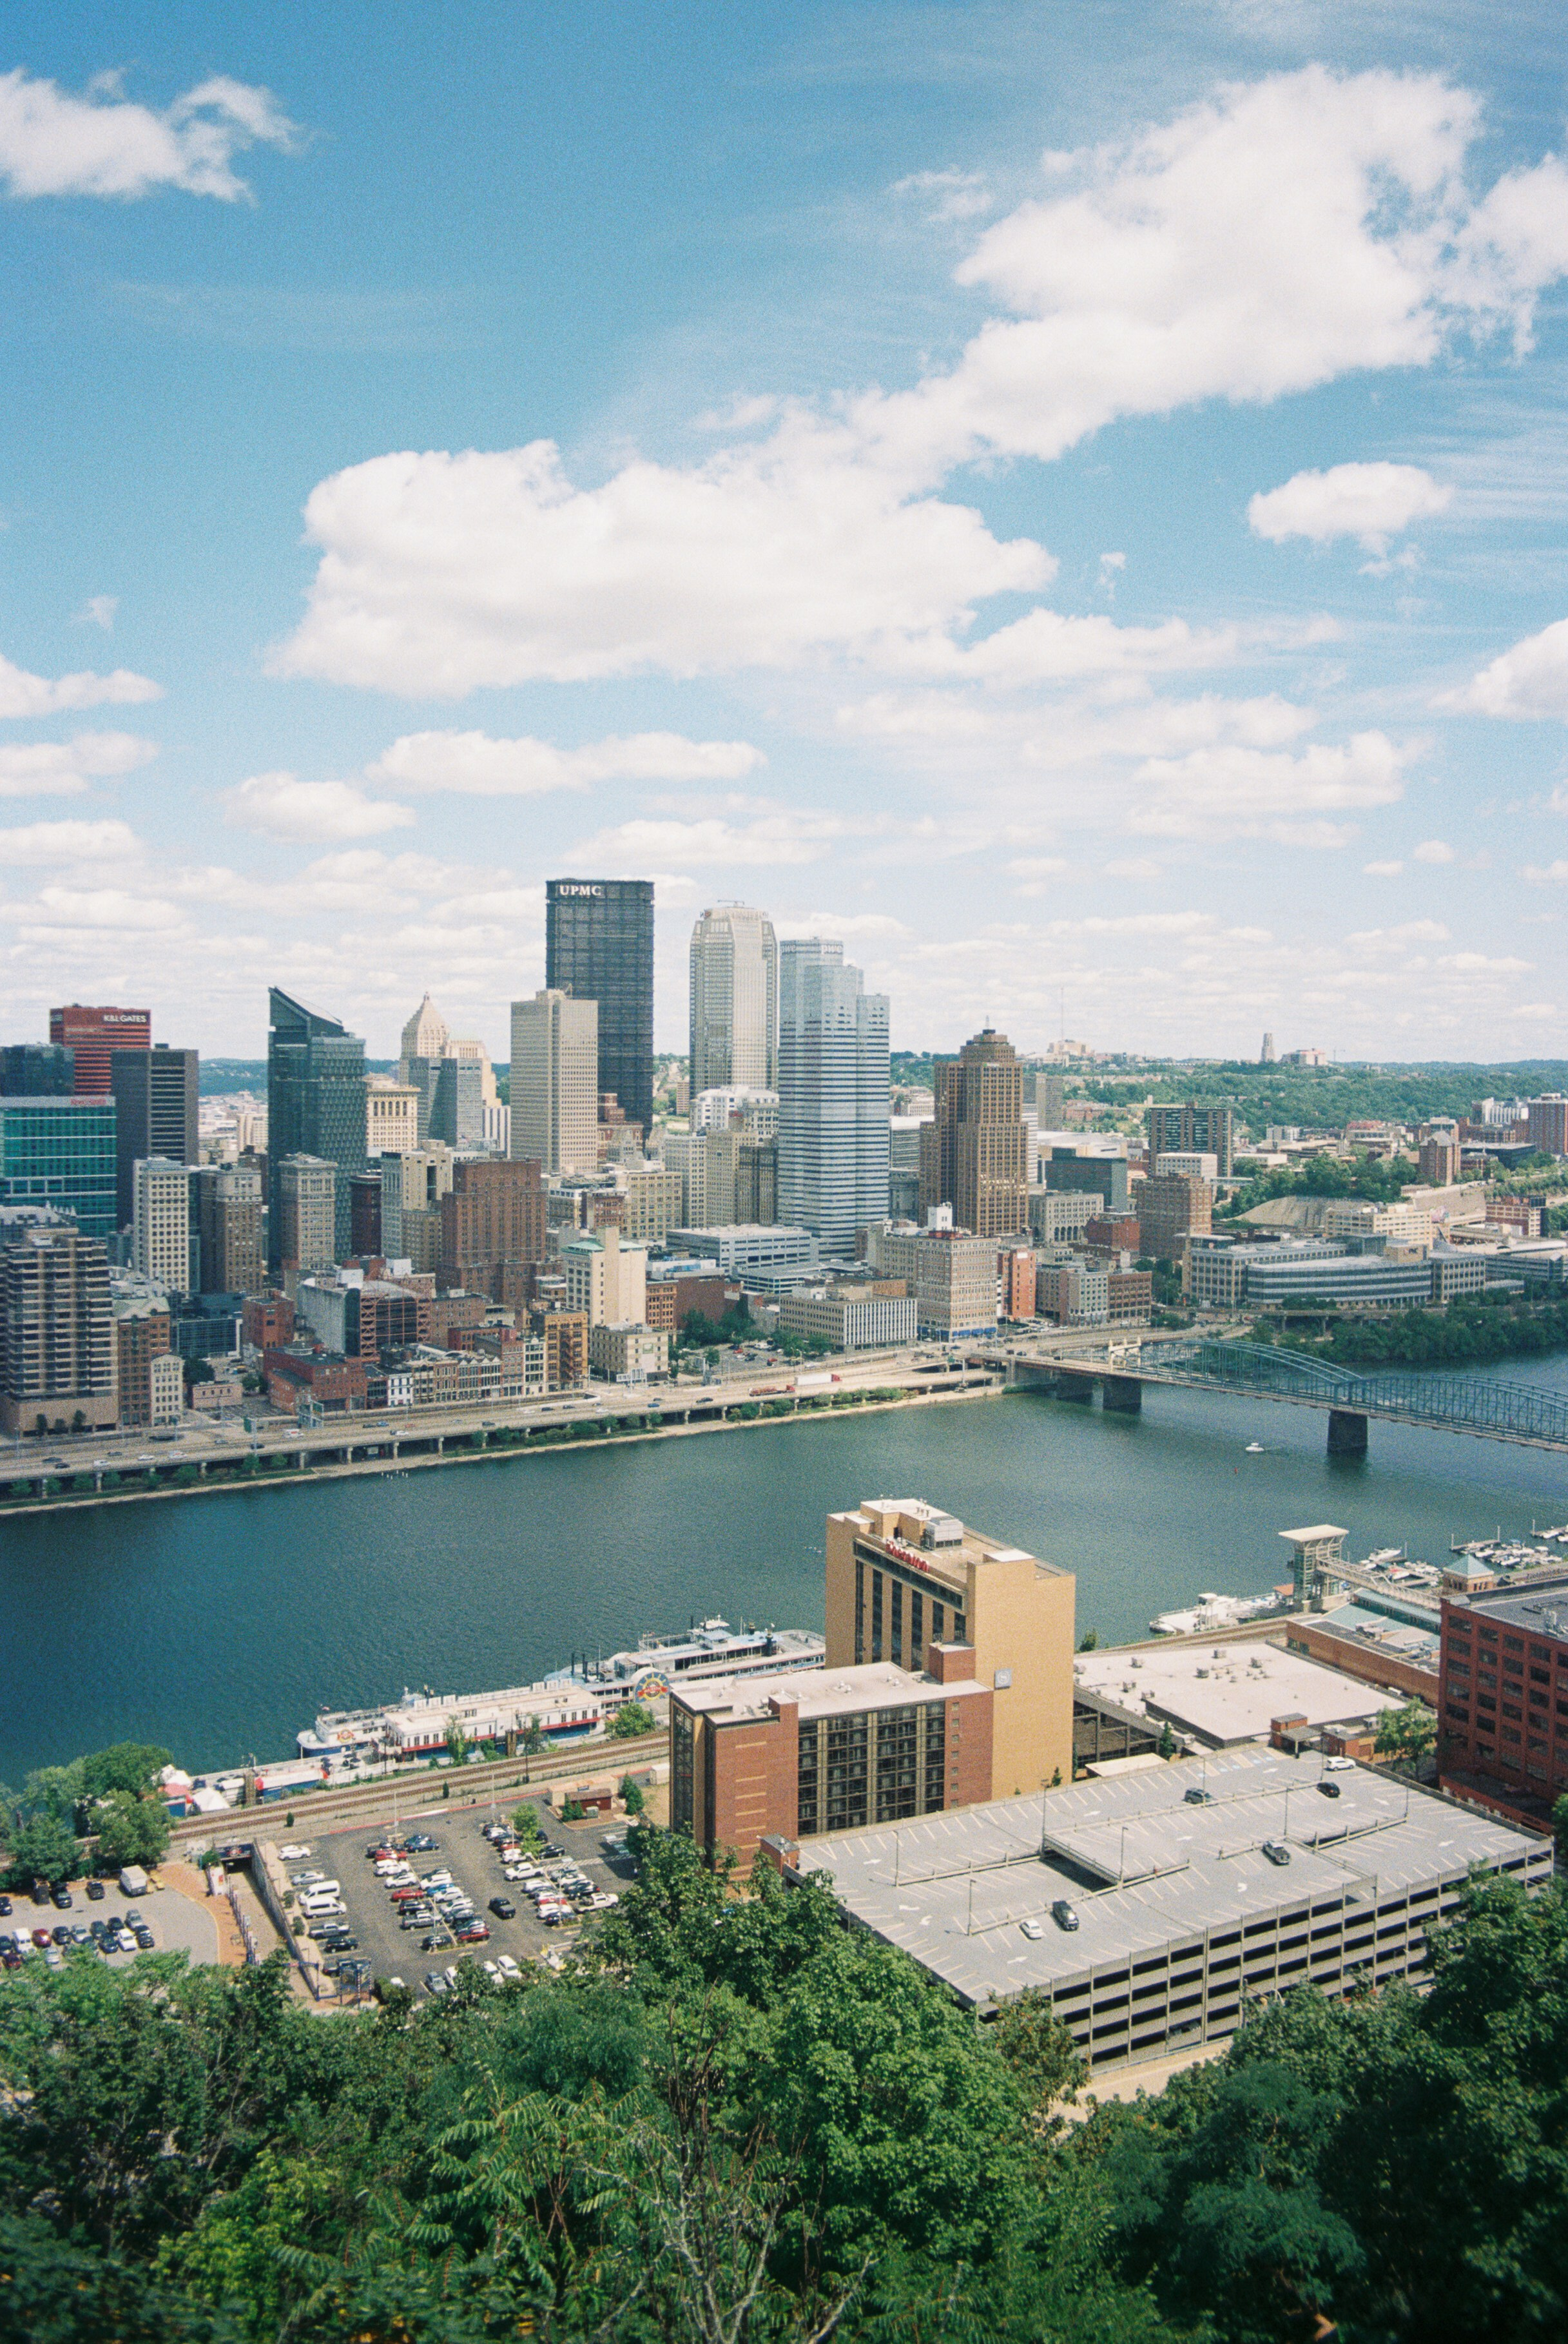
\includegraphics[scale=0.385]{./Images/banner.jpg}}} % Image background
\centering
\vspace*{5cm}
\par\normalfont\fontsize{35}{35}\sffamily\selectfont
\textbf{ECE358H1 Fall 2024}\\
{\LARGE Foundations of Computing}\par % Book title
\vspace*{1cm}
{\Huge Nasrudeen Oladimeji}\par % Author name
\endgroup

%----------------------------------------------------------------------------------------
%	COPYRIGHT PAGE
%----------------------------------------------------------------------------------------

\newpage
~\vfill
\thispagestyle{empty}

%\noindent Copyright \copyright\ 2014 Andrea Hidalgo\\ % Copyright notice

\noindent\textsc{University of Toronto}\\

\noindent \textsc{github.com/Nasr-905}\\ % URL

\noindent Professor: Andreas Veneris\\ % License information

\noindent \textit{First release, September 2024} % Printing/edition date

%----------------------------------------------------------------------------------------
%	TABLE OF CONTENTS
%----------------------------------------------------------------------------------------

\chapterimage{./Images/head1.jpg} % Table of contents heading image

\pagestyle{empty} % No headers

\tableofcontents % Print the table of contents itself

%\cleardoublepage % Forces the first chapter to start on an odd page so it's on the right

\pagestyle{fancy} % Print headers again

% theorem
% problem
% example
% vocabulary
% definition
% corollary
% remark
% proof
% lemma
% observation
% proposition
% claim
% fact
% assumption

\chapterimage{./Images/head2.jpg} % Chapter heading image
\chapter{The Introduction}
\section{Administrative Information}

\begin{itemize}
    \item Similar to ECE345, may be able to substitute lectures
    \item 5 homeworks, no extensions
    \item Textbook: CLRS (Cormen, Leiserson, Rivest, Stein)
    \item Course email: ece.algorithms+358@gmail.com
    \item Homework: 20\%
    \item \begin{itemize}
        \item Groups of 2-3
        \item You can switch Groups
    \end{itemize}
    \item Midterm: 30\%
    \item \begin{itemize}
        \item Open Textbook + Notes
    \end{itemize}
    \item Final: 45\%
    \item \begin{itemize}
        \item Open Textbook + Notes
    \end{itemize}
\end{itemize}

\section{Course Overview}
\begin{itemize}
    \item Background (Discrete Math, ~5 lectures): Asymptotic Analysis, recurrences, summations, graph/trees, permutation \& combinations
    \item Sorting (~4 lectures): Quick, Heap, Radix/Counting, Lower Bound
    \item Binary Search Trees (~3 lectures): Red-Black, searching min/max
    \item Hashing (~ 1 lecture)
    \item Greedy Algorithms (~2 lectures)
    \item Dynamic Programming (~2 lectures)
    \item \textbf{Midterm}
    \item Amoratized analysis \& splay trees (~3 lectures)
    \item Grph Algorithms (~3 lectures)
    \item \begin{itemize}
        \item Basic (~1 lecture)
        \item MSTs (~1 lecture)
        \item Shortest Paths (~1 lecture)
        \item Max Flow (~2 lecture)
    \end{itemize}
    \item History of Computations (~1 lecture)
    \item NP-Completeness (~5 lectures)
    \item Blockchain \& Cryptography (After hours)
\end{itemize}

\section{Asymptotics}
\begin{definition}
    {Big-O Notation, Upper Bound}
    We say that $f(n) = O(g(n))$ \textit{iff} $O(g(n)) = f(n): \exists$ positive constants $c$ and $n_0$ such that $0 \leq f(n) \leq c\times g(n)$ for all $n \geq n_0$
\end{definition}
% Functions c times g(n) upper bound, f(n), and h(n) lower bound are plotted using tikz 
\begin{figure}[H]
    \centering
    \begin{tikzpicture}
        \draw[->] (0,0) -- (10,0) node[right] {$n$};
        \draw[->] (0,0) -- (0,10) node[above] {$f(n)$};
        \draw[domain=0:10,smooth,variable=\x,blue] plot ({\x},{\x}) node[right] {$f(n)$};
        \draw[domain=0:10,smooth,variable=\x,red] plot ({\x},{0.5*\x}) node[right] {$g(n)$};
        \draw[domain=0:10,smooth,variable=\x,green] plot ({\x},{0.25*\x}) node[right] {$h(n)$};
    \end{tikzpicture}
\end{figure}
% add a dotted n_0 line near the origin (n_0) is small

Essentialy, we don't care about small value, we care about the upper bound of the functions $f(n)$ and $g(n)$ as $n$ approaches infinity.

\begin{example}
    \begin{align*}
        f(n) &= 3n + 7 \in O(n)\\
        13n + 7 &\leq 14n, n_0 = 7, c = 14
    \end{align*}
    We can see that $f(n)$ is bounded by $O(n)$ because $f(n) \leq c\times g(n)$ for all $n \geq n_0$. \\
    You can choose any $c$ and $n_0$ that satisfies the inequality.
\end{example}

\begin{example}
    \begin{align*}
        n! = 1\times 2 \times 3 \ldots n \leq n \times n \cdots n = O(n^n)\\
    \end{align*}
\end{example}

\begin{definition}
    {Big-$\Omega$ Notation, Lower Bound}
    We say that $f(n) = \Omega(h(n))$ \textit{iff} $O(h(n)) = f(n): \exists$ positive constants $c$ and $n_0$ such that $0 \leq c\times h(n) \leq f(n)$ for all $n \geq n_0$
\end{definition}

\begin{example}
    [Arithmetic Sequence]
    \begin{align*}
        1 + 2 + 3 + \cdots + n \geq (\frac{n}{2}) + (\frac{n}{2} + 1) + \cdots + (n) \geq \frac{n}{2}\times \frac{n}{2} = (c = \frac{1}{4}) - n^2 = \Omega(n^2), n_0 \geq 1
    \end{align*}
\end{example}

\begin{definition}
    {Big-$\Theta$ Notation, Tight Bound}
    We say that $f(n) = \Theta(g(n))$ \textit{iff} $O(g(n)) = f(n) \land \Omega(g(n)) = f(n)$
\end{definition}

\begin{example}
    \begin{align*}
        1 + 2 + 3 + \cdots + n = \frac{n(n+1)}{2} = 
        \frac{n^2}{2} + \frac{n}{2} + 1= \Theta(n^2)
    \end{align*}
\end{example}

\begin{example}
    [Summation]
    Show that $\sum_{i=1}^{n} i^k = \Theta(n^{k+1})$
    \begin{align*}
        \sum_{i=1}^{n} i^k & \leq \sum_{i=1}^{n} n^{k} = n^{k+1} = O(n^{k+1})\\
    \end{align*}
    Therefore, $\sum_{i=1}^{n} i^k = O(n^{k+1})$, now we need to show that $\sum_{i=1}^{n} i^k = \Omega(n^{k+1})$
    \begin{align*}
        2f(n) =& \sum_{i=1}^{n}i^k + \sum_{i=1}^{n}(n-i+1)^k  \\
        = & 1 + 2^k + 3^k + \cdots + n^k + n^k + (n-1)^k + \cdots + 1^k\\
    \end{align*}
    \begin{align*}
        \sum_{i=1}^{n} i^k & \geq \sum_{i=\frac{n}{2}}^{n} i^k \geq \sum_{i=\frac{n}{2}}^{n} (\frac{n}{2})^k = \frac{n}{2} \times (\frac{n}{2})^k = \frac{n^{k+1}}{2^{k+1}} = \Omega(n^{k+1})
    \end{align*}
\end{example}

\subsection*{Cookbook}
\begin{definition}
    [Transitivity]
    If $f(n) = \Theta(g(n))$ and $g(n) = \Theta(h(n))$, then $f(n) = \Theta(h(n))$
\end{definition}


\begin{definition}
    [Symmetry]
    \begin{align*}
        f(n) &= \Theta(g(n)) \text{ \textit{iff} } g(n) = \Theta(f(n)) \\
        f(n) &= O(g(n)) \text{ \textit{iff} } g(n) = \Omega(f(n))
    \end{align*}
\end{definition}

\begin{theorem}
    [Other Properties]
    \begin{align*}
        n^a & \in O(n^b) \text{ \textit{iff} } a \leq b\\
        \log_a(n) & \in O(\log_b(n)) \forall a, b \\
        c^n & \in O(d^n) \text{\textit{iff}} c \leq d \\
        \text{If } f(n) & \in O(g(n)) \text{ and } h(n) \in O(k(n)) \text{ then } f(n) + h(n) \in O(g(n) + k(n))\\
    \end{align*}
    
\end{theorem}

% \chapterimage{./Images/head3.jpg} % Chapter heading image
\chapter{Deterministic \& Randomized Algorithms}

\section{Asymptotics Contd.}
\begin{definition}
    [Monte Carlo Algorithms]
    A Monte Carlo algorithm is an algorithm that may return an incorrect answer with a small probability. The algorithm is said to be a Monte Carlo algorithm if it always runs in a fixed amount of time and the probability of returning an incorrect answer is at most $1/2$.
\end{definition}

\begin{definition}
    [Las Vegas Algorithms]
    A Las Vegas algorithm is an algorithm that always returns the correct answer. The algorithm is said to be a Las Vegas algorithm if it always runs in a fixed amount of time and the expected running time is finite.
\end{definition}

\begin{remark}
    In algorithms, we optimize time and memory usage. Memory is relatively cheap nowadays, so we can afford to use more memory. However, time is a very important factor. We can use randomness to reduce the time complexity of an algorithm.
\end{remark}
\subsection*{Time Complexity}
\begin{itemize}
    \item Best Case: The minimum time taken by the algorithm for an input size of $n$.
    \item Worst Case: The maximum time taken by the algorithm for an input size of $n$.
    \item Average/Expected Case: The average time taken by the algorithm for an input size of $n$.
    \item Amortized: The average time taken by the algorithm for a sequence of operations.
\end{itemize}

\section{Deterministic QuickSort}
\begin{definition}
    [QuickSort]
    QuickSort is a divide-and-conquer algorithm. It works as follows:
    \begin{enumerate}
        \item Choose a pivot element $p$ from the array.
        \item Partition the array into three parts: $L$ (elements less than $p$), $E$ (elements equal to $p$), and $G$ (elements greater than $p$).
        \item Recursively sort $L$ and $G$.
        \item Concatenate $L$, $E$, and $G$ to get the sorted array.
    \end{enumerate}
\end{definition}
% \begin{algorithm}[H]
%     \SetAlgoLined
%     \KwIn{Array $A$ of size $n$}
%     \KwOut{Sorted array $A$}
%     \If{$n \leq 1$}{
%         \Return $A$\;
%     }
%     $p \gets A[0]$\;
%     $L \gets \{x \in A \mid x < p\}$\;
%     $E \gets \{x \in A \mid x = p\}$\;
%     $G \gets \{x \in A \mid x > p\}$\;
%     \Return $\text{QuickSort}(L) + E + \text{QuickSort}(G)$\;
%     \caption{QuickSort}
% \end{algorithm}

\section{Logarithms}
\begin{definition}
    [Logarithm]
    \[
        \log_b a = c \iff b^c = a
    \]
    where $a, b, c \in \mathbb{R}$ and $b > 0, b \neq 1$.
\end{definition}
\begin{definition}
    [Properties of Logarithms]
    \begin{align*}
        \log_b 1                          & = 0                               \\
        \log_b b                          & = 1                               \\
        \log_b (a \cdot c)                & = \log_b a + \log_b c             \\
        \log_b \left( \frac{a}{c} \right) & = \log_b a - \log_b c             \\
        \log_b a^c                        & = c \cdot \log_b a                \\
        \log_b a                          & = \frac{1}{\log_a b}              \\
        \log_b(\frac{1}{a})               & = -\log_b a                       \\
        a^{\log_b c}                      & = c^{\log_b a}                    \\
        \log^(5)n                         & = \log(\log(\log(\log(\log(n)))))
    \end{align*}
\end{definition}

\begin{definition}
    [Iterated Logarithm]
    \[
        \log^(i) = \begin{cases}
            n                  & \text{if } i = 0 \\
            \log(\log^{(i-1)}) & \text{if } i > 0
        \end{cases}
    \]

\end{definition}

\begin{definition}
    \[\log^{*} n = \min \{ i \geq 0 \mid \log^{(i)} n \leq 1 \}\]
    A very slow-growing function.
\end{definition}

\begin{example}
    \[
        \log^{*} 2 = 1
    \]
    \[
        \log^{*} 2^2 = 1 + \log^{*} 2 = 2
    \]
    \[
        \log^{*} 2^4 = 3
    \]
\end{example}

\begin{definition}
    [Fibonacci Numbers]
    \[
        F_n = F_{n-1} + F_{n-2}
    \]
    \[
        F_0 = 0, F_1 = 1
    \]
    In terms of the golden ratio:
    \[
        F_n = \frac{\phi^n - \hat{\phi}^n}{\sqrt{5}}
    \]
\end{definition}

\begin{definition}
    [Golden Ratio]
    \[
        \phi = \frac{1 + \sqrt{5}}{2}
    \]
    \[
        \hat{\phi} = \frac{1 - \sqrt{5}}{2}
    \]
\end{definition}

\section{Summations}
\begin{definition}
    [Arithmetic Series]
    \[
        \sum_{i=1}^{n} i = \frac{n(n+1)}{2}
    \]
    \[
        \sum_{i=1}^{n} i^2 = \frac{n(n+1)(2n+1)}{6}
    \]
    \[
        \sum_{i=1}^{n} i^3 = \left( \frac{n(n+1)}{2} \right)^2
    \]
\end{definition}

\begin{definition}
    [Geometric Series]
    \[
        \sum_{i=0}^{n} a^i = \frac{a^{n+1} - 1}{a - 1}
    \]
    \[
        \sum_{i=0}^{\infty} a^i = \frac{1}{1 - a}
    \]
\end{definition}

\begin{definition}
    [Infinite Series]
    \[
        \sum_{i=0}^{\infty} x^k = \frac{1}{1 - x} \text{ when} |x| < 1
    \]
\end{definition}

\begin{example}
    [Summation]
    Show $ \sum_{k=0}^\infty kx^k = \frac{x}{(1-x)^2} $. \\
    You can differentiate both sides to prove this.
    \begin{align*}
        \sum x^k      & = \frac{1}{1-x} \quad \text{differentiate}     \\
        \sum kx^{k-1} & = \frac{1}{(1-x)^2} \quad \text{multiply by x} \\
        \sum kx^k     & = \frac{x}{(1-x)^2}
    \end{align*}

\end{example}

\subsection*{Telescoping Summation}
\begin{definition}
    [Telescoping Summation]
    \[
        \sum_{i=1}^{n} (a_i - a_{i-1}) = a_n - a_0 \quad \text{or} \quad \sum_{i=1}^{n} (a_i - a_{i+1}) = a_0 - a_n
    \]
\end{definition}

\begin{example}
    [Telescoping Summation]
    \[
        \sum_{k=1}^{n-1} \frac{1}{k+1} = \sum \frac{1}{k} - \frac{1}{k+1} = 1 - \frac{1}{n}
    \]
\end{example}

\begin{definition}
    [Bionomial Theorem]
    \[
        (x + y)^n = \sum_{k=0}^{n} \binom{n}{k} x^{n-k} y^k
    \]
    \[
        \binom{n}{k} = \frac{n!}{k!(n-k)!}
    \]
\end{definition}

% \chapter[short]{Mathematical Proofs}
\section{Proof by Induction}

\begin{theorem}
    [Principle of Mathematical Induction]
    The predicate $P(n)$ is true for all $n \geq 0$ if:
    \begin{align}
        \text{Basis: }          & P(0) \text{ is true since } 0 < 2^0 = 1. \\
        \text{Hypothesis: }     & P(k) \text{ is true for some } k \geq 0. \\
        \text{Inductive Step: } & P(k) \implies P(k+1).                    \\
    \end{align}

\end{theorem}

\begin{example}
    Show $n < 2^n$ for all $n \geq 0$.
    \begin{proof}
        \begin{itemize}
            \item Basis: $0 < 2^0 = 1$.
            \item Hypothesis: for $n$ that is we assume $n < 2^n$.
            \item Inductive Step: we prove $n+1 < 2^{n+1}$.
                  \begin{align*}
                      n+1 & < 2^n + 1 \text{ (by hypothesis)} \\
                          & < 2^n + 2^n = 2^{n+1}.
                  \end{align*}
        \end{itemize}
    \end{proof}
\end{example}

\begin{example}
    Prove the sum o fthe first $n$ odd numbers is $n^2$.
    \begin{proof}
        \begin{itemize}
            \item Basis: $1 = 1^2$.
            \item Hypothesis: for $n$ we assume $1 + 3 + \ldots + (2n-1) = n^2$.
            \item Inductive Step: we prove $1 + 3 + \ldots + (2n-1) + (2n+1) = (n+1)^2$.
                  \begin{align*}
                      1 + 3 + \ldots + (2n-1) + (2n+1) & = n^2 + 2n + 1 \\
                                                       & = (n+1)^2.
                  \end{align*}
        \end{itemize}
    \end{proof}
\end{example}

\begin{definition}
    [Power Set]
    The power set of a set $S$ is the set of all subsets of $S$. \\
    \textbf{Notation:} $2^S$.
\end{definition}

\begin{example}
    [Power Set]
    Let $S = {A, B, C}$. Then:
    \begin{align}
        2^S & = \{\emptyset, \{A\}, \{B\}, \{C\}, \{A, B\}, \{A, C\}, \{B, C\}, \{A, B, C\}\}.
    \end{align}
\end{example}

\begin{claim}
    [Power Set]
    The powerset of S, $2^S$, has $2^{|S|}$ elements.
\end{claim}
\begin{proof}
    \begin{itemize}
        \item Basis: $|S| = 1$ so $S = {A}$ and $2^S = \{\emptyset, A\}$, which has $2^1 = 2$ elements.
        \item Hypothesis: $|S| = n$ elements has $2^n$ elements.
        \item Inductive Step: $|S| = n+1$ elements has $2^{n+1}$ elements.
              \begin{align*}
                  2^{n+1} & = 2^n \cdot 2 = 2 \cdot 2^n.
              \end{align*}
        \item[] \textit{Imagine a set with $n$ elements, and we add one more, using combinatorics, we can see that one elements combined with all the subsets of the $n$ elements set will give us $2^n$ additional subsets.}
    \end{itemize}
\end{proof}

\begin{claim}
    [Chess Sets]
    Show that every $2^n \times 2^n$ chessboard with any one square removed can be tiled with $1\times1$ L-shaped tiles.
\end{claim}
\begin{proof}
    \begin{itemize}
        \item Basis: $2^0 \times 2^0$ chessboard is a $1\times1$ chessboard, which is already tiled.
        \item Hypothesis: $2^n \times 2^n$ chessboard can be tiled.
        \item Inductive Step: $2^{n+1} \times 2^{n+1}$ chessboard can be tiled.
              \begin{itemize}
                  \item Divide the $2^{n+1} \times 2^{n+1}$ chessboard into four $2^n \times 2^n$ chessboards.
                  \item Remove one square from the $2^{n+1} \times 2^{n+1}$ chessboard.
                  \item Remove the square that is not in the same $2^n \times 2^n$ chessboard as the removed square.
                  \item Tile the remaining $2^{n+1} \times 2^{n+1}$ chessboard.
              \end{itemize}
    \end{itemize}
\end{proof}

\section{Proof by Contradiction}
\begin{definition}
    [Proof by Contradiction]
    You get predicate $P(n)$ is true for all $n \geq 0$ by assuming that $P(n)$ is false for some $n \geq 0$ and deriving a contradiction.
\end{definition}

\begin{claim}
    if $x^2 - 5x + 4 < 0$ then $x > 0$.
\end{claim}
\begin{proof}
    \begin{itemize}
        \item Assume $x^2 - 5x + 4 < 0$ and $x \leq 0$.
        \item $x^2 - 5x + 4 < 0 \iff x^2 < 5x - 4 \iff x^2 < \text{some negative number}$.
        \item Which is a contradiction because $x^2$ is always positive.
    \end{itemize}
\end{proof}

\begin{claim}
    If $3n+2$ is odd then $n$ is odd.
\end{claim}

\begin{proof}
    \begin{itemize}
        \item Assume $3n+2$ is odd and $n$ is even.
        \item $n = 2k$ for some integer $k$.
        \item $3n+2 = 3(2k) + 2 = 6k + 2 = 2(3k+1) = $ an even number, a contradiction.
    \end{itemize}
\end{proof}

\begin{claim}
    $\sqrt{2}$ is irrational.
\end{claim}
\begin{proof}
    \begin{itemize}
        \item Assume $\sqrt{2}$ is rational.
        \item $\sqrt{2} = \frac{a}{b}$ for some integers $a$ and $b$.
        \item $2 = \frac{a^2}{b^2} \iff 2b^2 = a^2$.
        \item $a^2$ is even $\iff a$ is even.
        \item $a = 2k$ for some integer $k$.
        \item $2b^2 = (2k)^2 = 4k^2 \iff b^2 = 2k^2$.
        \item $b^2$ is even $\iff b$ is even.
        \item $\frac{a}{b}$ is not in lowest terms, a contradiction.
    \end{itemize}
\end{proof}

\begin{claim}
    If $a^2 = $ even, then $a$ is even.
\end{claim}
\begin{proof}
    \begin{itemize}
        \item Assume $a^2$ is even and $a$ is odd.
        \item $a = 2k+1$ for some integer $k$.
        \item $a^2 = (2k+1)^2 = 4k^2 + 4k + 1 = 2(2k^2 + 2k) + 1$.
        \item $a^2$ is odd, a contradiction.
    \end{itemize}
\end{proof}

\section{Permutations and Combinations}
\begin{definition}
    [Rule of Product]
    If there are $n_1$ ways to do task A and $n_2$ ways to do task B, then there are $n_1 \cdot n_2$ ways to do both tasks.
\end{definition}

\begin{definition}
    [Rule of Sum]
    If there are $n_1$ ways to do task A and $n_2$ ways to do task B, then there are $n_1 + n_2$ ways to do either task A or task B.
\end{definition}

\begin{example}
    Choose $2$ books, one from each: 5 Latin books, 7 Greek, 10 Frnech.
    \begin{itemize}
        \item $5 \cdot 7 = 35$ ways to choose a Latin and a Greek book.
        \item $5 \cdot 10 = 50$ ways to choose a Latin and a French book.
        \item $7 \cdot 10 = 70$ ways to choose a Greek and a French book.
        \item $35 + 50 + 70 = 155$ ways to choose two books.
    \end{itemize}

\end{example}
\section{Permutations}
\begin{vocabulary}
    $p(n,x) = $ number of ways to arrange $x$ objects out of $n$ when order matters. \\
    $p(n,x) = \frac{n!}{(n-x)!}$.
\end{vocabulary}

\begin{proof}
    [Permutations]
    \begin{itemize}
        \item There are $n$ ways to choose the first object.
        \item There are $n-1$ ways to choose the second object.
        \item There are $n-x+1$ ways to choose the $x$th object.
        \item There are $n \cdot (n-1) \cdot \ldots \cdot (n-x+1) = \frac{n!}{(n-x)!}$ ways to choose $x$ objects.
    \end{itemize}
\end{proof}
\begin{example}
    [In how many ways n people can sit around a circular table?]
    For a line, there are $p(n,n)$ ways to order a group of $n$ people, but in a circle, then the first person can either be in the front or back, so: $p(n,n) = \frac{n!}{(n-r)!} = (n-1)!$
\end{example}

\begin{theorem}
    []
    If not all objects are distinct, but we got:
    \begin{itemize}
        \item $q_1$ of the first kind
        \item $q_2$ of the second kind
        \item $q_k$ of the $k^{\text{th}}$ kind
    \end{itemize}
    Then: $\frac{n!}{q_1!q_2!\ldots q_k!}$
\end{theorem}

\begin{example}
    Five black balls and eight white balls can be arranged in:
    \[
        \frac{13!}{5!8!}
    \]
\end{example}

\begin{example}
    Show that $(k!)!$ is divisible by $(k!)^{(k-1)!}$ giving a combinatorical argument.
    \begin{itemize}
        \item $k$ of the first kind
        \item $k$ of the second kind
        \item $k$ of the $(k-1)!$ kind
    \end{itemize}
    $\therefore k(k-1)! = k!$ total
    \[
        \frac{(k!)!}{k!k!\ldots k!} = \frac{(k!)!}{(k!)^{(k-1)!}}
    \]
\end{example}

\begin{example}
    Among 10 billion numbers between $1, \ldots, 10,000,000,000$ how many contain the digit "$1$"? \\
    \textbf{Solution:} \\
    Think between $1, \ldots, 9,999,999,999$.\\
    There are $9$ ways to choose each digit, so $9^{10}$ numbers without the number $1$. There are $10^{10}$ total numbers \\
    So there are $10^{10} - 9^{10}$ numbers with the digit $1$.
    EDIT THIS, MIGHT BE INCORRECT
\end{example}

\section{Combinations}
\begin{definition}
    [Combinations]
    $c(n,r) = $ number of ways to choose $x$ objects out of $n$ when order does not matter. \\
    $c(n,r) = \frac{n!}{r!(n-r)!} = \frac{p(n,r)}{r!} = \left( \begin{matrix}
                n \\
                r
            \end{matrix} \right). $ \\
    $c(n,r) = c(n,n-r)$.
\end{definition}

\begin{example}
    In how many ways can three digit numbers be selected from a set containing numbers in the hundreds such that they're unique sum is divisible by $3$?
    \begin{itemize}
        \item $0 \mod 3$: $3 \cdot 3 \cdot 2 = 18$ ways.
        \item $1 \mod 3$: $3 \cdot 3 \cdot 3 = 27$ ways.
        \item $2 \mod 3$: $3 \cdot 3 \cdot 3 = 27$ ways.
        \item $18 + 27 + 27 = 72$ ways.
    \end{itemize}
    EDIT, THIS MIGHT BE INCORRECT
\end{example}

\begin{example}
    Eleven scientists are working on a secret project. They lock the docs into a cabinet that can open \textit{iff} at least $6$ of the scientists are present. \\
    a) What is the smallest # of locks needed for the cabinet \\
    b) What is the smallest # of keys each scientist need have? \\

    \textbf{Solution:} \\
    a) $c(11,5) = 462$ locks. \\
    b) $c(10,5) = 252$ keys. Because any scientist should be able to join any group of 5 to open the cabinet.
\end{example}

% \chapter{Recurrences}

\section{Recurrences}

\subsection{Merge Sort}
\begin{definition}
    [Merge Sort]
    \label{def:merge_sort}
    Merge sort is a divide-and-conquer algorithm that divides a list into two halves, recursively sorts the two halves, and then merges the sorted halves.\\
    The complexity of merge sort is $T(n) = 2T\left(\frac{n}{2}\right) + O(n)$
\end{definition}

% minted python for merge sort
\begin{minted}{python}
def merge_sort(A, p, r):
    if p < r:
        q = (p + r) // 2
        merge_sort(A, p, q) # T(n/2)
        merge_sort(A, q + 1, r) # T(n/2)
        merge(A, p, q, r) # O(n)
\end{minted}

\begin{figure}
    \centering
    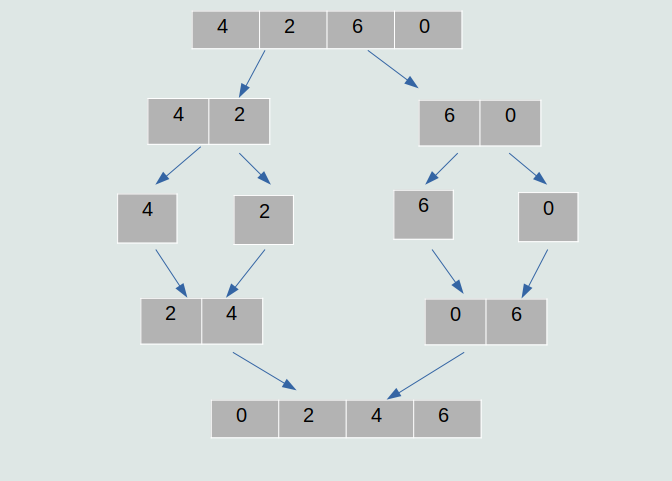
\includegraphics[width=0.5\textwidth]{./LECTURE_4/merge-sort.png}
\end{figure}

\begin{definition}
    [Master Method]
    \label{def:master_method}
    The master method is a general technique for solving recurrences of the form. \\
    Let $a \geq 1$ and $b > 1$ be constants, let $f(n)$ be a function, and let
    \[
        T(n) = aT\left(\frac{n}{b}\right) + f(n) \quad \text{has a solution}
    \]
    \begin{enumerate}
        \item If $f(n) = O(n^{\log_b a - \varepsilon})$ for some constant $\varepsilon > 0$, then $T(n) = \Theta(n^{\log_b a})$
        \item If $f(n) = \Theta(n^{\log_b a})$, then $T(n) = \Theta(n^{\log_b a} \log n)$
        \item If $f(n) = \Omega(n^{\log_b a + \varepsilon})$ for some constant $\varepsilon > 0$, and if $a f\left(\frac{n}{b}\right) \leq k f(n)$ for some constant $k < 1$ and sufficiently large $n$, then $T(n) = \Theta(f(n))$
    \end{enumerate}
    The master theorem will solve the recurrence of type $T(n) = aT\left(\frac{n}{b}\right) + f(n)$ in the case that $f(n)$ is a polynomial.
\end{definition}

\begin{example}
    Say $ a = 2, b = 2, f(n) = O(n)$, which case is this?\\
    \textbf{Solution:} This is case 2, where $f(n) = O(n^{\log_b a})$ for some constant.\\
\end{example}

\begin{example}
    $T(n) = 9T\left(\frac{n}{3}\right)$ \\
    $a = 9, b = 3, f(n) = O(n^{\log_39} = n^{2}), T(n) = \Theta(n^2)$\\
    This is case 2, where $f(n) = \Theta(n^{\log_b a})$
\end{example}

\begin{example}
    $T(n) = 3T\left(\frac{n}{4}\right) + n\log n$ \\
    $a = 3, b = 4, f(n) = n\log n, log_43 = 0.792$\\
    $f(n) = n\log n = \Omega(n^{\log_43 + \varepsilon})$ for $\varepsilon = 0.9$\\
    We got $3f(\frac{n}{4}) = 3\frac{n}{4}\log\frac{n}{4} \leq \frac{3}{4}n\log n$\\
    We pick $\varepsilon = 3/4$ so that $T(n) = \Theta(n\log n)$\\
    This is case 1, where $f(n) = O(n^{\log_b a - \varepsilon})$ for some constant $\varepsilon > 0$
\end{example}

\subsection{Substitution (Induction) Method}
\begin{remark}
    "Guess" the form of the solution and then use induction to prove it.
\end{remark}

\begin{example}
    [Substitution Method]
    \label{ex:substitution_method}
    $T(n) = 2T\left(\frac{n}{2}\right) + n$ We guess $T(n) = O(n\log n)$\\
    \textbf{Hypothesis:} Assume true for less than $n$, this is true $T(\frac{n}{2}) \leq c\frac{n}{2}\log\frac{n}{2}$\\
    \textbf{Step: }
    Due to the hypothesis, we have:
    \begin{align*}
        T(n)       & \leq 2c\frac{n}{2}\log\frac{n}{2} + n   \\
                   & = cn\log n - cn + n                     \\
                   & \leq cn\log n \quad \text{if } c \geq 1 \\
        \therefore & T(n) = O(n\log n)
    \end{align*}
    \begin{proof}
        [Eroneous Induction]
        Guess $T(n) = O(n)$. We \textbf{hypothesize} $T(\frac{n}{2}) \leq 2c\frac{n}{2}$\\
        \textbf{Step:}
        \begin{align*}
            T(n) & \leq 2c\frac{n}{2} + n \\
            \leq cn + n \leq (c + 1)n = c'n
        \end{align*}
        This is not true, as $c'$ is a completely different constant.\\
    \end{proof}
    \textbf{Basis:} \\
    $n = 1, T(1) = \leq c |\log n| = 0$ doesn't hold for $n = 1$\\
    $T(2) \leq 2 c \log 2 = 2c $ \\
    $T(4) \leq c 3 \log 3 = c3.0477$ \\
    $ \therefore \quad \text{we pick} \quad c \geq 3$
\end{example}

\begin{example}

    \begin{align*}
        T(n) & = T(\frac{n}{2}) + T(\frac{2n}{3}) + n \\
    \end{align*}
    Think of $T(n)$ as a work function, where the total work is $= hO(n)$ where $h$ is the height of the tree. \\
    \[
        \frac{2}{3}^h \times n  = 1 \iff h = \log_{\frac{3}{2}} n = O(n) \]
    total work $= O(n\log n)$
\end{example}

% \include{LECTURE_5/lecture_5.tex}

% \include{LECTURE_6/lecture_6.tex}

\end{document}